
\documentclass[border=5pt]{standalone}
\usepackage[utf8]{inputenc}
\usepackage[T1]{fontenc}
\usepackage{amsmath,amssymb}
\usepackage{tikz}
\usetikzlibrary{arrows.meta,shapes.misc,calc}
\renewcommand{\familydefault}{\sfdefault}
\tikzset{
  ptcross/.style={cross out,draw,thick,minimum size=1.6mm,inner sep=0pt},
  vec/.style={->,thick,>={Stealth[length=2.6mm]}},
  vecu/.style={vec,color=blue!70!black},
  vecv/.style={vec,color=red!75!black},
  vecw/.style={vec,color=green!45!black},
  grid/.style={gray!35,thin},
}
\newcommand{\Vj}[1]{\overrightarrow{\text{#1}}}
\newcommand{\pt}[4]{\node[ptcross] at (#1,#2) {}; \node[anchor=#4,inner sep=2pt] at (#1,#2) {$#3$};}
\begin{document}
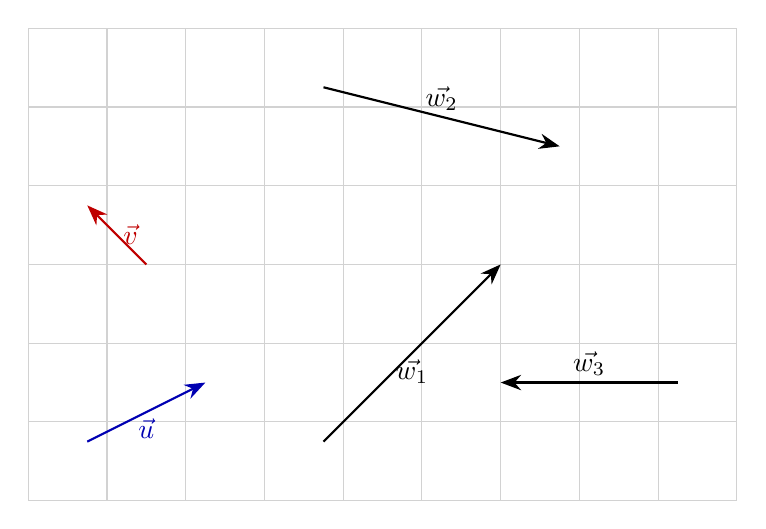
\begin{tikzpicture}[x=0.75cm,y=0.75cm]
\draw[grid] (0,0) grid (12,8);
\draw[vecu] (1,1) -- (3,2) node[midway,below=1pt,inner sep=1pt] {$\vec u$};
\draw[vecv] (2,4) -- (1,5) node[midway,right=1pt,inner sep=1pt] {$\vec v$};
\draw[vec] (5,1) -- (8,4) node[midway,below=1pt,inner sep=1pt] {$\vec{w_1}$};
\draw[vec] (5,7) -- (9,6) node[midway,above=1pt,inner sep=1pt] {$\vec{w_2}$};
\draw[vec] (11,2) -- (8,2) node[midway,above=1pt,inner sep=1pt] {$\vec{w_3}$};

\end{tikzpicture}
\end{document}
